\chapter[Metodologia]{Metodologia}

\section{Metodologia de Desenvolvimento de Software}

Um processo ou metodologia de desenvolvimento de software é uma coleção de atividades e resultados relacionados que auxiliam na criação de software. Por exemplo, análise e codificação de requisitos são duas das muitas atividades associadas. \cite{Soares2004}

Há vários tipos de metodologia de desenvolvimento de software como o Scrum, PMBOK, Kanban, Ágil, Ciclo de Vida Único, Modelo em cascata, entre outras. Cada uma delas possui suas próprias características e abordagens para gerenciamento de projetos, mas todas elas visam ajudar as equipes a entregar projetos de software de qualidade dentro do prazo, orçamento e com as funcionalidades esperadas. Algumas metodologias são mais estruturadas e baseadas em fases, enquanto outras são mais flexíveis e baseadas em fluxo de trabalho, o que torna importante escolher a metodologia mais adequada para o projeto específico. \cite{SilvaAnd2013}

\subsection{Metodologia Ágil}

As metodologias ágeis são um conjunto de abordagens para gerenciamento de projetos que se concentram em fornecer flexibilidade, adaptabilidade e colaboração entre equipes. Elas foram desenvolvidas originalmente para o desenvolvimento de software, mas agora são amplamente utilizadas em muitos outros campos. \cite{Libardi2010}

\subsubsection{Scrum}

Scrum é uma metodologia ágil específica que foi projetada para ajudar equipes a gerenciar projetos de desenvolvimento de software complexos e altamente incertos. Ele se concentra em entregar valor rapidamente e incrementos regulares, enquanto a equipe colabora e se adapta a mudanças no projeto. \cite{STOPA2019}

\subsubsection{Kanban}

Kanban é uma metodologia que se concentra em tornar visível o fluxo de trabalho, limitando o número de tarefas em andamento e permitindo que a equipe se adapte às mudanças de forma flexível. Ele é amplamente utilizado em conjunto com outras metodologias ágeis, como Scrum, para ajudar a equipe a aumentar a eficiência e a entrega de valor. \cite{Lage2008}

\subsection{Metodologia de Desenvolvimento Utilizada}

Kanban e Scrum são ambas metodologias ágeis, mas possuem abordagens diferentes para o gerenciamento de projetos. Enquanto o Scrum é uma metodologia mais estruturada e baseada em sprints, Kanban é uma metodologia mais flexível e baseada no fluxo de trabalho. Ambos têm seus próprios benefícios e podem ser usados de forma complementar para ajudar a equipe a alcançar seus objetivos de projeto. \cite{Kniberg2010}

Sendo assim, o projeto foi desenvolvido utilizando ambas as metodologias, Kanban e Scrum, para que fosse possível atingir os objetivos propostos. O Kanban foi utilizado para gerenciar o fluxo de trabalho, enquanto o Scrum foi utilizado para gerenciar as sprints.

\section{Ferramentas Utilizadas}

\subsection{Gerenciamento do Projeto}

\subsubsection{Trello}

Trello é uma plataforma que auxilia equipes a organizarem e priorizarem projetos. Utiliza quadros de tarefas, onde cada tarefa é representada por um cartão, que pode ser movido e organizado em listas para indicar o progresso e o estado do projeto. Ele é uma ferramenta útil para gerenciar tarefas do projeto, estabelecer prazos e definir prioridades, além de acompanhar o andamento de cada Sprint.

\subsubsection{Slack}

Slack é uma ferramenta de comunicação de equipe que permite que as equipes criem canais de bate-papo para discutir projetos, compartilhar arquivos e se comunicar de forma rápida e eficiente.

No contexto do desenvolvimento de software, Slack pode ajudar a equipe a se comunicar de forma mais eficiente e colaborativa, permitindo que desenvolvedores, gerentes de projetos e outros membros da equipe discutam e compartilhem informações de forma rápida e fácil. Ele pode ser usado para discutir problemas técnicos, atribuir tarefas, acompanhar o progresso do projeto e compartilhar arquivos, tudo em um único lugar. Além disso, ele pode ser integrado com outras ferramentas, como o GitHub, o Google Drive e o Trello, para ajudar a equipe a automatizar tarefas e trabalhar de forma mais eficiente.

\subsubsection{Google Drive}

Google Drive é um serviço de armazenamento e compartilhamento de arquivos na nuvem fornecido pelo Google. Ele permite que os usuários armazenem arquivos, como documentos, fotos e vídeos, e compartilhem esses arquivos com outras pessoas. Ele também oferece recursos de colaboração, como edição em tempo real de documentos, comentários e histórico de versões.

\subsection{Desenvolvimento}

\subsubsection{Figma}

Figma é uma ferramenta de design colaborativo que permite que equipes criem e compartilhem arquivos de design. Ele permite que os usuários criem protótipos de aplicativos e sites, além de permitir que eles compartilhem esses protótipos com outras pessoas para que possam colaborar e fazer comentários. Ele também permite que os usuários criem e compartilhem arquivos de design, como imagens, ícones e paletas de cores, que podem ser usados por outros membros da equipe.

\subsubsection{GitHub e GitHub Actions}

GitHub é uma plataforma de desenvolvimento de software que permite que os desenvolvedores armazenem, rastreiem e colaborem em projetos de código-fonte. Ele é baseado no sistema de controle de versão Git, que permite que os desenvolvedores façam alterações no código e versionem essas alterações, facilitando a colaboração e o controle de versão.

GitHub Actions é uma ferramenta de automação de fluxo de trabalho do GitHub. Ele permite que os desenvolvedores criem scripts de trabalho automatizados, chamados ``Ações'', que podem ser disparados por eventos, como o envio de código para o repositório ou a criação de uma nova issue. Isso permite automatizar tarefas comuns, como compilação, teste e implantação, e integrar com outras ferramentas, como ferramentas de integração contínua e de monitoramento de desempenho.

\subsubsection{Docker}

Docker é uma plataforma de virtualização de aplicativos que permite que os desenvolvedores embalem e distribuam facilmente aplicativos em contêineres. Um contêiner é uma forma de isolamento de sistemas operacionais que permite que um aplicativo seja embalado com todas as suas dependências, bibliotecas e configurações, de forma que possa ser executado de forma consistente em diferentes ambientes.

Docker permite que os desenvolvedores criem e gerenciem contêineres, e que esses contêineres sejam implantados em diferentes ambientes, incluindo computadores locais, nuvens públicas e privadas. Isso permite que os desenvolvedores criem aplicativos de forma mais eficiente e confiável, e que esses aplicativos possam ser executados de forma consistente em diferentes ambientes. Além disso, ele também permite a colaboração entre equipes, e aumenta a segurança, escalabilidade e gerenciamento do aplicativo.

\subsubsection{Visual Studio Code}

VSCode (Visual Studio Code) é um editor de código-fonte desenvolvido pela Microsoft. Ele é uma ferramenta gratuita e de código aberto, que suporta diversas linguagens de programação, incluindo JavaScript, Python, C++, Java e muitas outras. Ele oferece recursos avançados de edição, como sugestão de código, depuração e gerenciamento de versão. Além disso, ele também possui uma ampla variedade de extensões e plugins desenvolvidos pela comunidade, que podem ser usadas para adicionar recursos adicionais, como integração com ferramentas de teste, análise de código e integração com outras ferramentas.

\section{Definição de Escopo e Requisitos}

A definição de escopo e requisitos é uma etapa crítica no processo de gerenciamento de projetos, pois estabelece as expectativas e restrições do projeto, bem como os objetivos e entregáveis esperados.

O escopo do projeto é o conjunto de tarefas, atividades e entregáveis que precisam ser realizados para completar o projeto de acordo com as necessidades do cliente. Ele também inclui os limites e restrições do projeto, como tempo, orçamento e recursos disponíveis. A definição do escopo do projeto é importante para garantir que todos os envolvidos tenham uma compreensão clara do que é e não é incluído no projeto. \cite{Xavier2009}

Os requisitos são as necessidades e expectativas do cliente e do usuário final que devem ser atendidas pelo projeto. Eles são usados para guiar o desenvolvimento do projeto e incluem tanto requisitos funcionais (o que o sistema deve fazer) quanto requisitos não funcionais (como desempenho, segurança e usabilidade). A definição de requisitos é importante para garantir que o projeto entregue o valor esperado para o cliente e usuário final. \cite{Machado2018}

Em resumo, a definição de escopo e requisitos é importante para garantir que o projeto seja entregue dentro do prazo, orçamento e com as funcionalidades esperadas, e que ele atenda as necessidades do cliente e usuário final.

\subsection{Definição de Escopo}

Para a definição de escopo do projeto, foi realizada uma pesquisa com os alunos da UnB, que foram convidados a responder um questionário sobre suas experiências com o aprendizado de Python. Os resultados da pesquisa foram usados para definir o escopo do projeto, e também para definir os requisitos do projeto.

\subsubsection{Pesquisa com Alunos da UnB}

A pesquisa consistiu de duas perguntas, que foram respondidas por 22 alunos. A primeira pergunta perguntava quais eram as maiores dificuldades que os alunos encontraram ao aprender Python, e a segunda pergunta perguntava quais recursos ou características eles acreditavam que uma ferramenta de ensino de Python deve ter para ser eficaz. Os resultados da pesquisa estão apresentados na Tabela \ref{tab:pesquisa}.

\begin{longtable}{| p{.45\textwidth} | p{.45\textwidth} |}
    \hline
    \textbf{Quais são as maiores dificuldades que você encontrou ao aprender Python?} & \textbf{Quais recursos ou características você acredita que uma ferramenta de ensino de Python deve ter para ser eficaz?} \\ \hline
    Encontrar algumas bibliotecas não muito conhecidas ainda, além de suas documentações / orientações & ``Integrações nativas com bibliotecas já conhecidas de Python, facilitando automações (Como por exemplo o Jupyter). \\ \hline
    Seria muito bom se houvesse mais conteúdo sobre webscrapping com python em páginas dinâmicas (que sempre atualizam seus resultados) e as devidas ferramentas facilitadoras para o aprendizado do mesmo, mostrando texto e imagens de como foi feito em algum outro lugar. & Uma trilha real de um back-end. Ensinando os conceitos iniciais até o deploy. \\ \hline''
    Saber o que cada método faz, especificamente, e também, por onde começar um projeto: lib que usar e etc & Ter uma interface simples;  Recompensas por atividades resolvidas (exercicios); Vídeos curtos e objetivos; Ranking entre os alunos que está mandando bem; Dica ou trechos de livros para explicar aquele problema que foi proposto. \\ \hline
    Foi em entender a programar de forma Pythonic & Talvez auto-identação no começo seja interessante pra quem veio de linguagens com escrita parecida ao C \\ \hline
    Decorators, self, **kwargs. Não entendia bem como vinha informação desses caras, se não era objeto, não era passado por parametro, não tinha um super, me deu uma bugada legal na época & Acredito que recurso da visibilidade de um input virando um output e cases relacionados. Exemplo, supondo a função soma em que dois valores são somados, não somente os inputs e os outputs mas como a linguagem “enxerga” isso e entrega o valor. A partir disso, levantar pontos sobre “o que e um número” “o que e uma soma” “como a máquina enxerga isso” até a apresentação do dado. \\ \hline
    Quando chegou a parte de orientação a objeto e sempre tentar manter o código “pythonico” uma vez que a linguagem pede pra não termos códigos muito grandes, repetitivos e sem padrões & Exemplos claros e funcionais e balões de dicas quando se está indo para o caminho inverso \\ \hline
    Colocar em prática códigos funcionais de forma lógica & Plataforma de dúvidas remota e online, e exercícios de prática resolvidos passo a passo de diversas maneiras para que se possa estudar e analisar as diversas formas de chegar em um mesmo resultado \\ \hline
    Entraves psicológicos criados durante a graduação em relação a programação. Infelizmente, cheguei na faculdade sem saber nada e não tive suporte, além de um péssimo professor que aplicava medo e não ensinava direito & Acho que a prática. É sempre muito bom quando a gente vê um comando e em seguida implementamos ele de uma maneira meio que criativa. Tipo, ao mostrar como funciona um loop, seria legal tem um espaço pra praticar um loop podendo colocar outros comandos dentro dele. \\ \hline
    Acredito que por ter um background com outras linguagens, aprender python foi muito simples. & Aprofundamento em cada assunto \\ \hline
    Acho que a maneira com que a linguagem é apresentada pros calouros é de uma maneira bastante equivocada. & Exercícios de prática \\ \hline
    Lembrar de todos os comandos e suas aplicações & Praticidade, linguagem simples e de fácil acesso ao usuário \\ \hline
    Memorizar funções específicas, por exemplo a função de limitar a quantidade de dígitos decimais de uma variável. & Uma documentação simples, clara e direta, que explique de maneira concisa a forma mais eficiente de se resolver um problema proposto. \\ \hline
    Sinceramente, eu acredito que Python seja uma das linguagens de programação mais simples de estudar. No entanto, até o momento, tenho dificuldade em entender funções recursivas e funções anônimas (lambda). & Deve ter a presença de prática a cada conceito novo introduzido, por mais ínfimo que seja ele. No aprendizado é importante dominar o simples pra poder passar pro avançado. Um grande erros de vários professores, por exemplo, é apresentar (em aulas longuíssimas e maçantes puramente teóricas com slides infinitos, etc...) e cobrar assuntos avançados e mais complexos sem que os alunos tenham dominado plenamente os conceitos prévios que são mais básicos, simples e necessários para compreender os mais avançados.  De acordo com vários estudos pedagógicos, o aprendizado ativo (prática propriamente dita) é a melhor forma de reter o conhecimento, então a prática a cada conceito novo precisa ser frequente e constante na plataforma. \\ \hline
    A dificuldade de encontrar aulas rápidas objetivas que vão direto ao ponto sem enrolação & A melhor ferramenta, para o ensino de qualquer coisa, se chama, 'um bom professorª'. Outras coisas, como IDE, computador tal, são acessórios. Aliás, falando em acessórios, um SSD, é algo muito bom. \\ \hline
    ``Independente da linguagem, acho que uma de minhas maiores dificuldades, foi na 'memorização' dos códigos. Não que, memorizar a sintaxe da linguagem, seja exigido pelo mercado de trabalho. Mas, na disciplina de APC, por exemplo, nas provas, não era permitido consulta. Então, de certa forma, os alunos precisavam ter, parte da linguagem memorizada, no caso Python. & Debugger \\ \hline
    Além disso, eu mesmo, nunca gostei me memorizar nada. Sempre achei, que o importante, é a pessoa ser capaz, de processar a informação, seja ela qual for. Decorar e repetir, até papagaio faz! & Explicar passo a passo os comandos e não só lotar os alunos de comando sem explicar direito cada um \\ \hline
    Eu sempre gostei, de ver os resultados dos meus estudos, aplicados no mundo real. Depois de APC, os alunos pegam uma disciplina, chamada ED(Estrutura de Dados). A maioria dos alunos, nunca fizeram um CRUD na vida, uma página com HTML/CSS, JavaScript ou qualquer outra coisa prática com programação. Se deixar, os alunos saem do curso, sem estarem preparados pro mercado de trabalho. É lógico que a base que a universidade dá, é importante, eu só acho que falta um pouco mais de equilíbrio, entre teoria e prática. O mesmo equilíbrio é necessário em outras disciplinas, por exemplo, as de matemática.'' & Ajudar com a lógica de programação (inclusive loops e condições),  apontar erros de sintaxe, auxiliar no básico da linguagem como variáveis e tipos básicos \\ \hline
    Abstração & projetos práticos \\ \hline
    Algumas expressões que não são tão auto explicativas e pra saber colocar elas do jeito certinho para o código rodar & Ensinar lógica computacional antes de qualquer coisa, ter um ambiente simples e intuitivo, exercícios práticos e conectado com o cotidiano. \\ \hline
    Achei uma linguagem bem tranquila! A sintaxe não é tão detalhista quanto em outras linguagens, e a parada da indentação ajuda bastante a visualizar o código e a execução. As mensagens de erro também são mais concisas e claras & Didática, eficiência, facilidade \\ \hline
    colocar a mão na massa, aprender é fácil, o problema é a prática & ~ \\ \hline
    Não saber lógica computacional, decorar a sintaxe, fazer exercícios desconectados da realidade, não saber usar a documentação. & ~ \\ \hline
    Professora não se importava com todos, só com quem já sabia a linguagem. No primeiro dia de aula lembro que foi dito que não era necessário saber nada de programação, que todos avançariam igualmente mas é a maior mentira pregada, se você não saber pelo menos o básico você se roda, as dificuldades não são sanadas, as dúvidas comuns não eram levadas a sério. Enfim, só provando mais a ainda o elitismo da unb e as altas taxas de evasão dos cursos de TI de lá. & ~ \\ \hline
    \caption{Pesquisa de dificuldades e características de ferramentas no aprendizado de Python}
    \label{tab:pesquisa}
\end{longtable}

\subsubsection{Nuvem de palavras dos resultados da pesquisa}

Abaixo é apresentado uma nuvem de palavras com as respostas da primeira pergunta da pesquisa, que foi: \textit{Quais são as principais dificuldades que você teve ao aprender Python?}.

\begin{figure}[h]
    \centering
    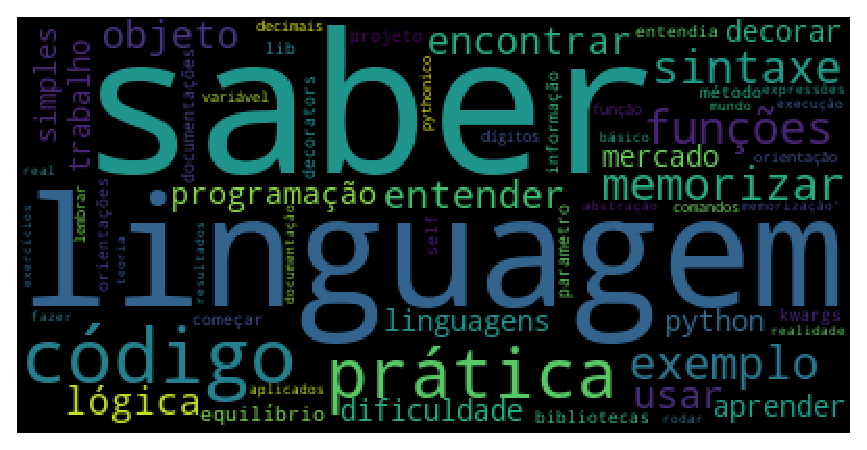
\includegraphics[width=0.8\textwidth]{figuras/nuvem_dificuldades.eps}
    \caption{Nuvem de palavras dos resultados da pesquisa}
    \label{nuvem_dificuldades}
\end{figure}

Abaindo é apresentado uma nuvem de palavras com as respostas da segunda pergunta da pesquisa, que foi: \textit{Quais são as principais dificuldades que você teve ao aprender Python?}.

\begin{figure}[h]
    \centering
    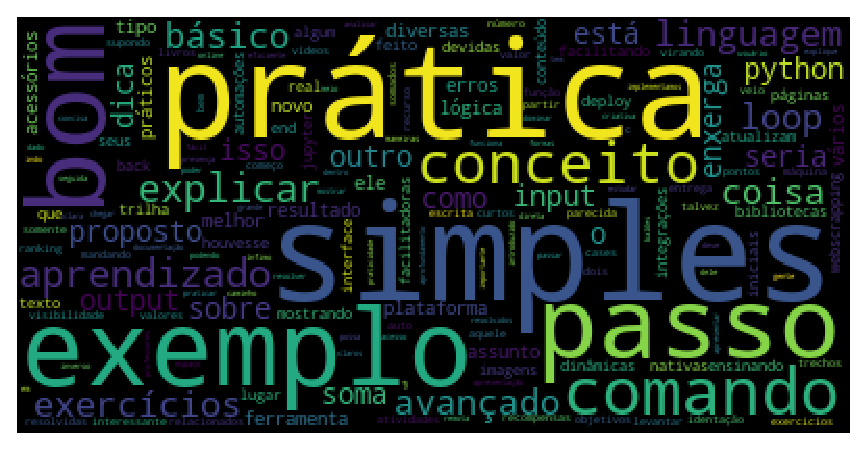
\includegraphics[width=0.8\textwidth]{figuras/nuvem_ferramentas.eps}
    \caption{Nuvem de palavras dos resultados da pesquisa}
    \label{nuvem_ferramentas}
\end{figure}

\subsection{Definição de Requisitos}

Os requisitos do projeto foram definidos com base nas necessidades identificadas na pesquisa. Os requisitos foram divididos em funcionais e não funcionais, e foram priorizados de acordo com a sua importância para o projeto.

\subsubsection{Requisitos Funcionais}

\begin{itemize}
    \item RF01 - Criação de conta: a plataforma deve permitir que os alunos criem uma conta para acessar os recursos da plataforma.
    \item RF02 - Visualização de projetos: a plataforma deve permitir que os alunos visualizem os projetos disponíveis na plataforma.
    \item RF03 - Execução de projetos: a plataforma deve permitir que os alunos executem os projetos disponíveis na plataforma.
    \item RF04 - Criação de projetos: a plataforma deve permitir que os alunos criem seus próprios projetos.
    \item RF05 - Visualização de quizzes: a plataforma deve permitir que os alunos visualizem os quizzes disponíveis na plataforma.
    \item RF06 - Submissão de quizzes: a plataforma deve permitir que os alunos submetam suas respostas para os quizzes disponíveis na plataforma.
    \item RF07 - Visualização de desafios: a plataforma deve permitir que os alunos visualizem os desafios disponíveis na plataforma.
    \item RF08 - Pontuação: ao criar um projeto ou submeter um quiz, o aluno deve receber uma pontuação.
    \item RF09 - Ranking: a plataforma deve permitir que os alunos visualizem um ranking com os usuários com mais pontos.
\end{itemize}

\subsubsection{Requisitos Não Funcionais}

\begin{itemize}
    \item RNF01 - Ambiente de aprendizado interativo: a plataforma deve oferecer um ambiente de aprendizado interativo e lúdico para os alunos, com a possibilidade de criação de jogos 2D.
    \item RNF02 - Responsividade e acessibilidade: a plataforma deve ser projetada para funcionar em diferentes navegadores.
    \item RNF03 - Segurança: a plataforma deve ser segura, com criptografia de dados e autenticação de usuários.
    \item RNF04 - Escalabilidade: a plataforma deve ser escalável, suportando um grande número de usuários.
    \item RNF05 - Manutenibilidade: a plataforma deve ser projetada para facilitar a manutenção e evolução do sistema.
    \item RNF06 - Usabilidade: a plataforma deve ser projetada para ser intuitiva e fácil de usar.
\end{itemize}

\subsection{Prova de Conceito}

Para garantir a viabilidade da solução imaginada, criou-se uma aplicação web simplificada que faz uso do Pyodide e do PixiJS. Seu objetivo foi o de oferecer um editor de texto integrado, com o qual o usuário pudesse executar código python e interagir com a aplicação resultante. A aplicação permitiu o desenho de figuras geométricas de tamanhos e cores variadas dentro de um canvas.

O design da aplicação não foi uma preocupação, uma vez que seu principal objetivo era o de comprovar a viabilidade.

\subsubsection{Referencial Tecnológico}

No apêndice \ref{apendice:referencial_tecnologico_poc} encontra-se o referencial tecnológico da aplicação de Prova de Conceito.

\subsubsection{Arquitetura da Aplicação}

No apêndice \ref{apendice:arquitetura_poc} encontra-se a arquitetura da aplicação de Prova de Conceito.

\subsubsection{Resultados}

No apêndice \ref{apendice:resultados_poc} encontra-se os resultados da aplicação de Prova de Conceito.

